\documentclass[a4paper,10pt]{report}
\usepackage[french]{babel}
\usepackage[utf8]{inputenc}
\usepackage[left=2.5cm,top=2cm,right=2.5cm,nohead,nofoot]{geometry}
\usepackage{url}
\usepackage{graphicx}

\linespread{1.1}



\begin{document}

\begin{titlepage}
\begin{center}
\textbf{\textsc{UNIVERSIT\'E LIBRE DE BRUXELLES}}\\
%\textbf{\textsc{Faculté des Sciences}}\\
%\textbf{\textsc{Département d'Informatique}}
\vfill{}\vfill{}
\begin{center}{\Huge Rapport : Villo !}\end{center}{\Huge \par}
\begin{center}{\large Pierre Gérard, Titouan Christophe}\end{center}{\Huge \par}
\vfill{}\vfill{} \vfill{}
\begin{flushleft}{\large \textbf{INFO-H-303 Base de données}}\hfill{Esteban Zimányi, Michaël Waumans}\end{flushleft}{\large\par}
\vfill{}\vfill{}\enlargethispage{3cm}
\textbf{Année académique 2014~-~2015}
\end{center}
\end{titlepage}

%\begin{abstract}
%Ce rapport présente ...
%\end{abstract}


\tableofcontents


\chapter{Diagramme entité association}
\section{Diagramme}
\begin{figure}[hbt]
  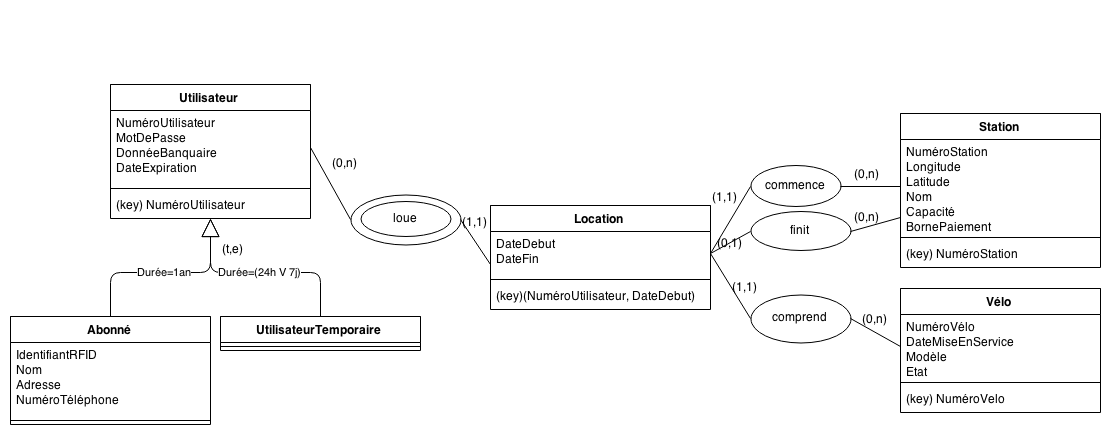
\includegraphics[scale=0.4]{dia/diagramme-entite-association.png}
  \caption{Diagramme entité association
}
\end{figure}
\section{Contraintes}
Les contraintes sont les suivantes :
\begin{itemize}
  \item La DateDebut d'une Location doit précéder la DateFin 
  \item La DateMiseEnService d'un Vélo doit précéder la DateDebut de sa Location
  \item La DateExpiration d'un Utilisateur doit précéder la DateDebut de sa Location
  \item La DateExpiration d'un Utilisateur doit précéder la DateFin de sa Location
  \item Un Vélo ne peut pas être loué deux fois en même temps
  \item Un Utilisateur ne peut pas faire deux Locations en même temps
  \item TODO \ldots
  % capacité ? 
\end{itemize}
\section{Hypothèses et justifications}

\chapter{Modèle relationnel}
\section{Modèle}

% ca cté du bo latek une fois
\begin{description}
\item[] \textbf{Utilisateur}(\underline{NuméroUtilisateur}, MotDePasse, DonnéeBanquaire, DateExpiration)

\item[] \textbf{Abonné}(IdentifiantRFID, Nom, Adresse, NuméroTélephone)
	% ICI herirtage ? Une des trois solution proposé

\item[] \textbf{UtilisateurTemporaire}()
	%ICI heritage ?

\item[] \textbf{Location}(\underline{NuméroUtilisateur,DateDebut},\textit{DateFin}, NuméroStationDépart , NuméroStationFin, NuméroVélo) % par sur de la notation pour NuméroStationDépart ???
	\begin{description}
	\item[] NuméroUtilisateur référence Utilisateur.NuméroUtilisateur
	\item[] NuméroVélo référence Vélo.NuméroVélo
	\item[] NuméroStationDépart référence Station.NuméroStation
	\item[] NuméroStationFin référence Station.NuméroStation
	\end{description}
	
\item[] \textbf{Station}(\underline{NuméroStation}, Longitude, Latitude, Nom, Capacité, BornePaiement)

 \item[] \textbf{Vélo}(\underline{NuméroVélo}, DateMiseEnService, Modèle, Etat)

\end{description}

\section{Contraintes}
\section{Hypothèses et justifications}




\end{document}